\documentclass[10pt,twocolumn,letterpaper]{article}

\usepackage{statcourse}
\usepackage{times}
\usepackage{epsfig}
\usepackage{graphicx}
\usepackage{amsmath}
\usepackage{amssymb}

% Include other packages here, before hyperref.

% If you comment hyperref and then uncomment it, you should delete
% egpaper.aux before re-running latex.  (Or just hit 'q' on the first latex
% run, let it finish, and you should be clear).
\usepackage[breaklinks=true,bookmarks=false]{hyperref}


\statcoursefinalcopy


\setcounter{page}{1}
\begin{document}


%%%%%%%%%%%%%%%%%%%%%%%%%%%%%%%%%%%%%%%%%%%%%%%%%%%%%%%%%%%%%%%
% DO NOT EDIT ANYTHING ABOVE THIS LINE
% EXCEPT IF YOU LIKE TO USE ADDITIONAL PACKAGES
%%%%%%%%%%%%%%%%%%%%%%%%%%%%%%%%%%%%%%%%%%%%%%%%%%%%%%%%%%%%%%%



%%%%%%%%% TITLE
\title{Forecasting Stock Returns via Supervised Learning}

\author{Samuel Ilic\\
{\tt\small ilic@wisc.edu}
\and
Second Author\\
{\tt\small secondauthor@wisc.edu}
\and
Third Author\\
{\tt\small thirdauthor@wisc.edu}
}

\maketitle
%\thispagestyle{empty}



% MAIN ARTICLE GOES BELOW
%%%%%%%%%%%%%%%%%%%%%%%%%%%%%%%%%%%%%%%%%%%%%%%%%%%%%%%%%%%%%%%


%%%%%%%%% ABSTRACT
\begin{abstract}
   The abstract for your project goes here. The length of the abstract
   should be between 200-250 words. Tips for writing a good abstract
   can be found at \url{https://writing.wisc.edu/Handbook/presentations_abstracts.html}.
\end{abstract}

%%%%%%%%% BODY TEXT
\section{Introduction}

This template is based on the CVPR conference template\footnote{\url{http://statcourse2018.thecvf.com/submission/main_conference/author_guidelines}}.

The information in this template is very minimal, and this file should serve you as a framework for writing your report. You may prefer to use a more collaboration-friendly tool while drafting the report with your class mates before you prepare the final report for submission. Remember that you should \textbf{submit both the report and code} you used for this project via Canvas. Also, \textbf{only one member per team} needs to submit the project material.


This is an example of a mathematical equation:

$$f(\mathbf{x}; \mathbf{w}) = \sum_{i=1}^{n} w_ix_i.$$

This is a mathematical expression, $h(\mathbf{x}) = \hat{y}$ formatted in text. 

The project report should be 6-8 pages long (not counting references)
and should contain the sections that are already provided in this paper. Please
check out the text in these sections for further information.


\subsection{Subsection}

You can use paragraphs or subsections to further structure your
main sections. This is an example of a subsection.

\paragraph{This is a paragraph title.} This is an example of a paragraph.

\section{Related Work}

Related work should be discussed here. This is an example of a citation \cite{mirjalili2018gender}. To format the citations properly, put the
corresponding references into the bibliography.bib file. You can obtain
BibTeX-formatted references for the "bib" file from Google Scholar 
(\url{https://scholar.google.com}), for example, by clicking on the 
double-quote character under a citation and then selecting \mbox{"BibTeX"} as
shown in Figure \ref{fig:google-scholar-1col} and 
Figure \ref{fig:google-scholar-2col}.

\begin{figure}[t]
\begin{center}
   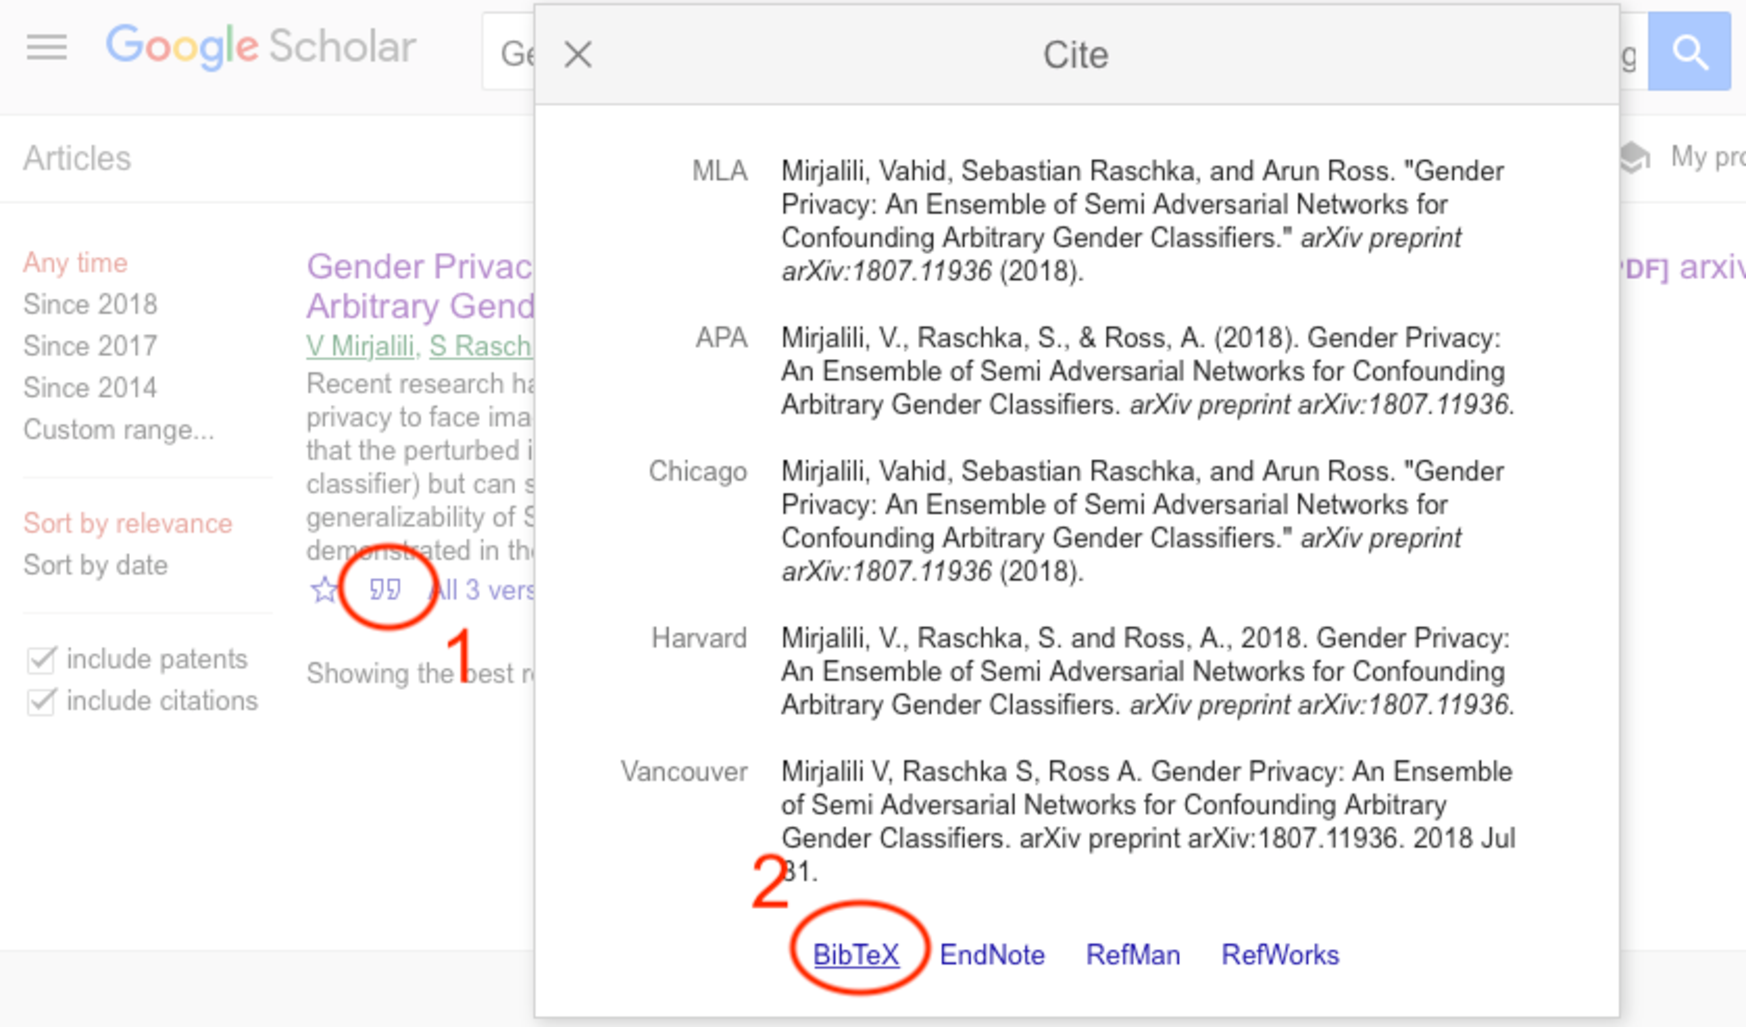
\includegraphics[width=0.8\linewidth]{Figures/google-scholar.pdf}
\end{center}
   \caption{Example illustrating how to get BibTeX references from
   Google Scholar as a 1-column figure.}
\label{fig:google-scholar-1col}
\end{figure}


\begin{figure*}
\begin{center}
   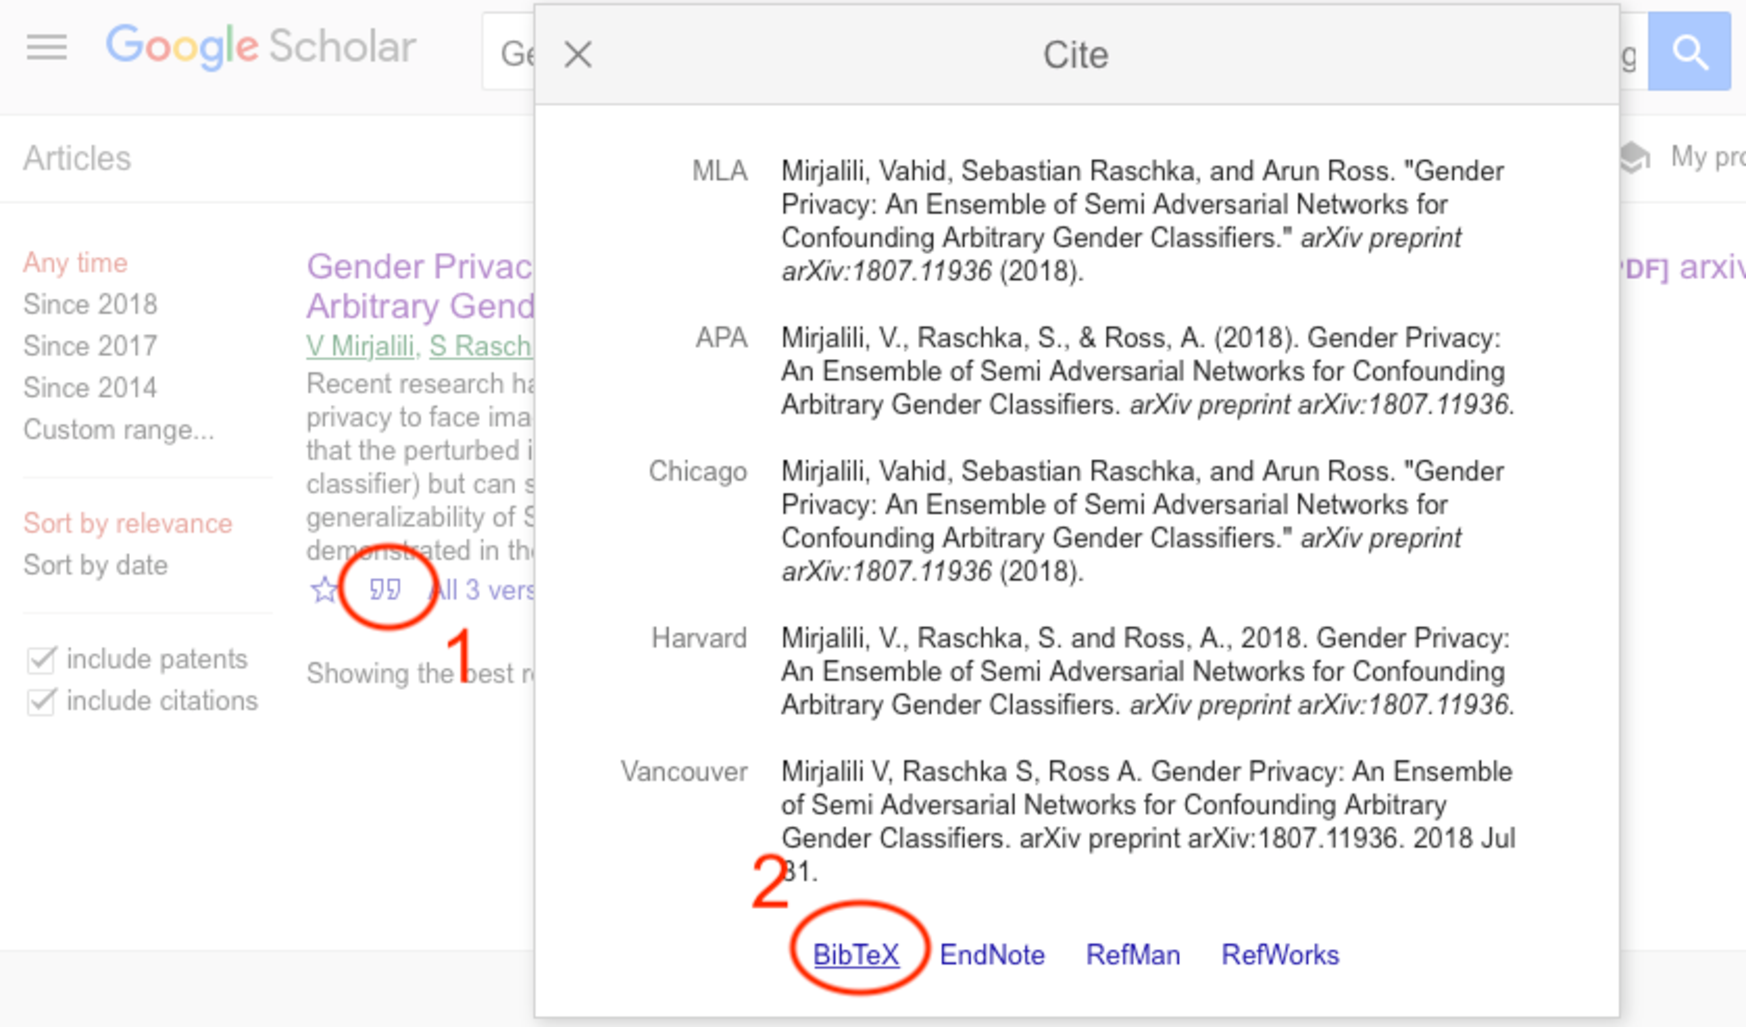
\includegraphics[width=0.8\linewidth]{Figures/google-scholar.pdf}
\end{center}
   \caption{Example illustrating how to get BibTeX references from
   Google Scholar as a 2-column figure.}
\label{fig:google-scholar-2col}
\end{figure*}

Table \ref{tab:some-table} shows an example for formatting a table.

\begin{table}
\begin{center}
\begin{tabular}{|l|c|}
\hline
Method & Accuracy \\
\hline\hline
Method 1 & $70 \pm 3$ \% \\
 Method 2 & $76 \pm 3$ \% \\
\hline
\end{tabular}
\end{center}
\label{tab:some-table}
\caption{This is an example of a table.}
\end{table}


\section{Proposed Method}

Describe the method(s) you are proposing, developing, or using. I.e., details
of the algorithms may be included here. 

\section{Experiments}

Describe the experiments you performed. You may want to create separate
subsections to further structure this section.

\subsection{Dataset}

Briefly describe your dataset in a separate subsection.


\subsection{Software}

Briefly list (and cite) software software you used.

\subsection{Hardware}

If relevant, list hardware resources you used.


\section{Results and Discussion}

Describe the results you obtained from the experiments and interpret them.
Optionally, you could split "Results and Discussion" into two separate
sections.

\section{Conclusions}

Describe your conclusions here. If there are any future directions, you can
describe them here, or you can create a new section for future directions.

\section{Acknowledgements}

List acknowledgements if any. For example, if someone provided you a dataset, or
you used someone else's resources, this is a good place to acknowledge
the help or support you received.

\section{Contributions}

Describe the contributions of each team member who worked on this project.


{\small
\bibliographystyle{ieee}
\bibliography{bibliography.bib}
}

\end{document}
